\documentclass[conference]{IEEEtran}
\IEEEoverridecommandlockouts
\usepackage{cite}
\usepackage{amsmath,amssymb,amsfonts}
\usepackage{algorithmic}
\usepackage{flafter}
\usepackage{graphicx}
\usepackage{textcomp}
\usepackage{xcolor}
\def\BibTeX{{\rm B\kern-.05em{\sc i\kern-.025em b}\kern-.08em
    T\kern-.1667em\lower.7ex\hbox{E}\kern-.125emX}}

\begin{document}

\title{Actividad G.1\\Pila de DatoOs
}

\author{\IEEEauthorblockN{Ricardo David López Arellano}
\IEEEauthorblockA{\textit{Departamento de Ingeniería en Computación} \\
\textit{CUCEI}\\
Universidad de Guadalajara\\
ricardo.lopez1361@alumnos.udg.mx}
}

\maketitle

\begin{abstract}
El \textit{abstract} es un resumen de la actividad que debe tener entre 100 y 300 palabras, como máximo.
\end{abstract}

\begin{IEEEkeywords}
Las palabras clave deben ser relativas a la actividad, mínimo cuatro.
\end{IEEEkeywords}

\section{Originalidad}

   Me comprometo a producir trabajo académico íntegro, lo que significa un trabajo que se adhiere a los estándares intelectuales y académicos de atribución exacta de las fuentes, uso y recolección de datos apropiados, y transparencia en el reconocimiento de las contribuciones de las ideas, descubrimientos, interpretaciones y conclusiones de otros.

   Acepto que la trampa en los exámenes, el plagio o la fraudulenta representación de las ideas o lenguaje de otros como propio, la falsificación de datos o cualquier otra instancia de deshonestidad académica, violan los estándares de LA MATERIA, así como los estándares del mundo en general en el campo del conocimiento y las relaciones.

%\begin{center}
% \vspace{0.5cm}
% \makebox[8cm]{\hrulefill}
% Firma
%\end{center}

\section{Introducción}

   Este documento es un reporte para \LaTeX...

\section{Tema 1}

...

\section{Tema 2}

\subsection{Subtema 1}

   Lista de ejemplo.

\begin{itemize}
\item Elemento 1.
\item Elemento 2.
\item Elemento 3.
\item Elemento 4.
\end{itemize}

\subsection{Ecuaciones}

\begin{equation}
 a+b=\gamma
 \label{ecuacion: efecto cuerpo}
\end{equation}
donde $a$ es la ...

\subsection{Figuras y Tablas}

   En la Tabla \ref{tabla: ejemplo 1} se muestra ...

\begin{table}
\caption{Tablas}
\begin{center}
\begin{tabular}{cccc}
\hline
\textbf{Table}&\multicolumn{3}{c}{\textbf{Table Column Head}} \\
\cline{2-4} 
\textbf{Head} & \textbf{\textit{Table column subhead}}& \textbf{\textit{Subhead}}& \textbf{\textit{Subhead}} \\
\hline
copy& More table copy$^{\mathrm{a}}$& &  \\
\hline
\multicolumn{4}{l}{$^{\mathrm{a}}$Sample of a Table footnote.}
\end{tabular}
\label{tabla: ejemplo 1}
\end{center}
\end{table}

   En la Fig. \ref{figura: senoidal} se presenta una señal senoidal, la cual ...

\begin{figure}
\centering
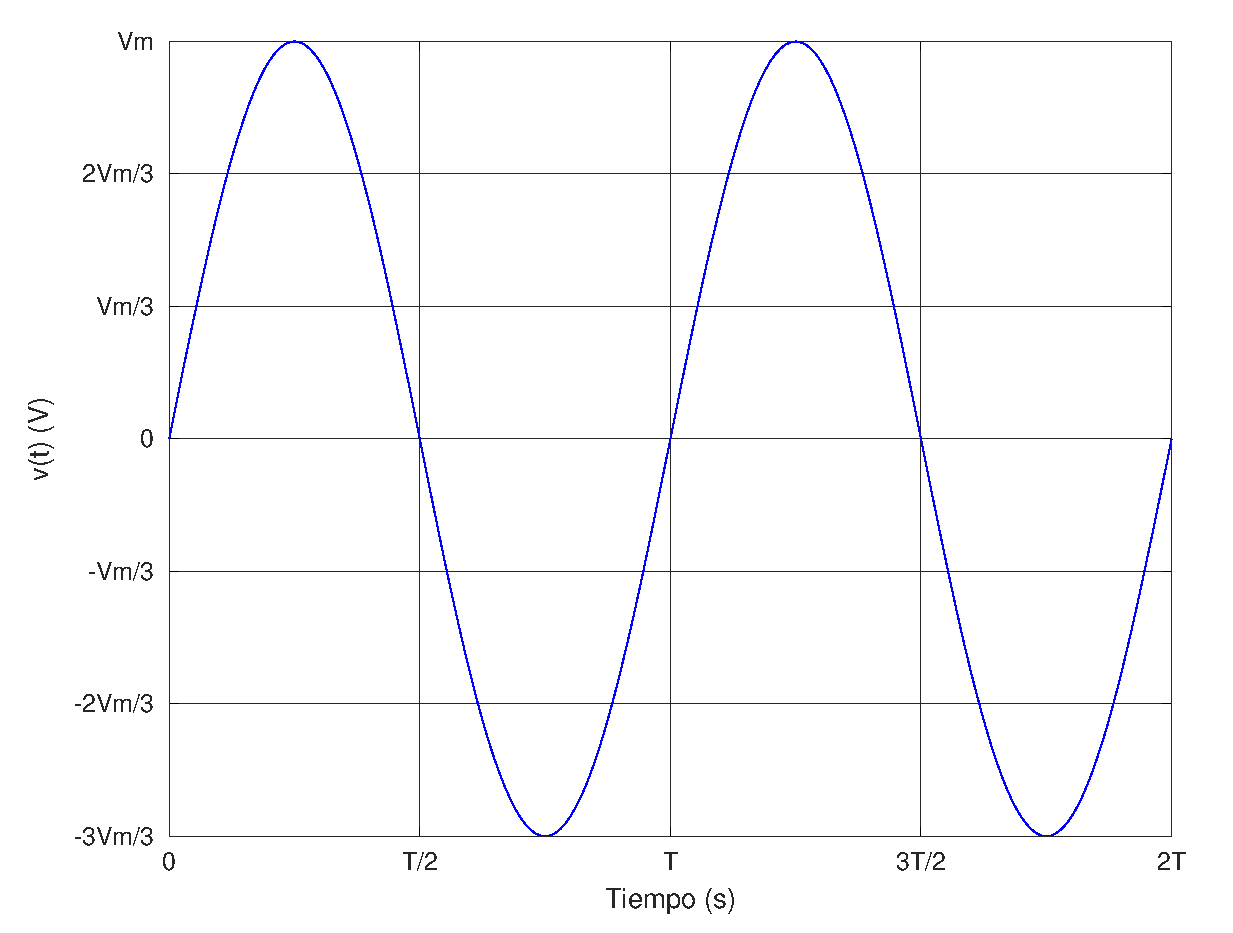
\includegraphics[width=0.5\textwidth]{senoidal.eps}
\caption{Señal senoidal.}
\label{figura: senoidal}
\end{figure}

\section*{Agradecimientos}

   Aquí se deben poner los agradecimientos.

\section*{Referencias}

   Las referencias deben ir de acuerdo a los documentos utilizados para la elaboración de la actividad, utilizando el formato de IEEE. Poniendo en primer lugar la primer referencia utilizada \cite{eason1955}.

\begin{thebibliography}{00}
\bibitem{eason1955} G. Eason, B. Noble, and I. N. Sneddon, ``On certain integrals of Lipschitz-Hankel type involving products of Bessel functions,'' Phil. Trans. Roy. Soc. London, vol. A247, pp. 529--551, April 1955.
\bibitem{maxwell1892} J. Clerk Maxwell, A Treatise on Electricity and Magnetism, 3rd ed., vol. 2. Oxford: Clarendon, 1892, pp.68--73.
\bibitem{jacobs1963} I. S. Jacobs and C. P. Bean, ``Fine particles, thin films and exchange anisotropy,'' in Magnetism, vol. III, G. T. Rado and H. Suhl, Eds. New York: Academic, 1963, pp. 271--350.
\end{thebibliography}

\end{document}
